\section{Problem Formulation} \label{section:problem_formulation}
The resource-constrained project scheduling problem (RCPSP) is a strongly NP-hard algorithmic problem \cite{RN20} where the objective is to minimise makespan (overall required time to finish all tasks). 

RCPSP is about a project consisting of a set of tasks \(N\) which all have to be completed to finish the project. Each task \(i\) has a duration \(d_i\) and requires an amount \(r_{i,k}\) of a resource type \(k\). A project provides a set of limited resource types \(R\) to process tasks each with an availability \(a_k\) constant throughout the project horizon. Tasks can be scheduled in timeslots as long as the overall resource type requirement does not exceed the provided amount at any time. Furthermore, a (possible empty) set of task pairs \((i,j)\) defines precedence relations \(A\) where \(i\) has precedence over \(j\). The task pairs have a finish-start type precedence meaning that a task must be completed entirely before its successor can be started. Some additional assumptions are that each resource type required by any task is provided \(k\in R\), no single task will require more of a resource type than provided \(r_{i,k}\leq a_k\) and a worst-case scenario makespan called the horizon \(T\) is given by the sum of all task durations.

This project structure can be modelled as an activity-on-the-node network (where activity also means task) \(G=(N, A)\). The network is extended with 2 dummy tasks that model the start and finish of the project. These dummy tasks have a duration of 0 and no resource requirement. The makespan can now be defined as the starting time of the finish dummy task. An example project network can be seen at the top of figure \ref{figure:figure1}.

\subsection{PRCPSP-ST}
The RCPSP definition can be extended in different ways including task preemption and setup times. All previous proposed and researched extensions have been surveyed and summarised in a paper \cite{RN6, RN27}.

Preemption allows an activity to be paused after it has been started by the project. A preempted task in a schedule is like multiple individual tasks that each represent a segment of the original task. Preemption is only allowed at integer points of the task duration. Tasks might be preempted at any fraction of the duration but the infinite ways to split a task make defining an algorithm much harder. A solution to approximate fractional preemption is rescaling the time units used project. When hours are scaled down to minutes for example, a task can be preempted on each minute instead of on the hour approaching a possible required granularity. Figure \ref{figure:figure1} shows a non-preemptive and preemptive schedule for an example project.

Setup time \(s\) is introduced to try and prevent tasks from being split into many impractical segments. This prevention is done by adding additional processing time (setup time) to task segments that start after a previous segment has been preempted. During the setup time, the same amount and type of resources are required as the task itself. By penalizing preemption in this way algorithms will only introduce split tasks when the makespan can be improved in a meaningful way.

\begin{figure}
	\centering
    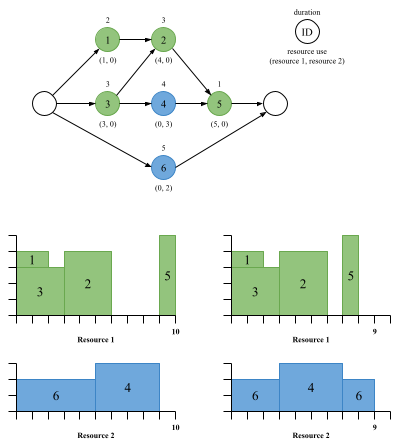
\includegraphics[width=0.5\textwidth]{PRCPSP-ST.png}
    \caption{An example project network (top), non-preemptive schedule (left) and preemptive schedule with makespan reduction (right)}
	\label{figure:figure1}
\end{figure}

\subsection{Related Work}
Algorithms for both preemption and the inclusion of setup times have been proposed and researched in earlier work.

For pre-emption, a branch-and-bound procedure was used to show that task preemption did not reduce the makespan of projects by a significant amount \cite{RN21}. A zero-one integer programming approach was used to solve projects with preemption under multiple objectives \cite{RN54}. Colouring techniques were used to produce optimal preempted schedule results \cite{RN55}. Later, meta-heuristic approaches were shown to be effective on preemption-based scheduling with linear programming algorithms \cite{RN57, RN56}. The branch-and-bound was researched again but this time allowing parts of tasks to be scheduled in parallel called fast-tracking \cite{RN7}. This fast-tracking did show a more significant reduction in makespan at the cost of the problem becoming more complicated. The introduction of preemptive scheduling to the multi-mode variant of the RCPSP has also been studied \cite{RN61, RN59, RN60}.

Setup times have been introduced for task segments after preemption before \cite{RN13}. The setup times can be modelled in different ways and are summarized in an overview paper \cite{RN62}. The fast-tracking method used for preemptive scheduling also included setup times after a task is split \cite{RN7}.

Newer research showed that even without fast-tracking preempted tasks can sometimes lead to a makespan reduction contrary to previous research \cite{RN1}. It also showed that when this reduction is possible it does not require many splits in the project tasks. This motivates further research into the PRCPSP-ST problem variant if having a lower makespan is profitable enough to have tasks not be finished once it is started. The algorithm used to show that makespan reductions are possible is meta-heuristic and does not provide proven optimal solutions. When having a lower makespan is critical enough to sacrifice tasks being completed in one go it might be reasonable to require the schedule to be the most optimal it can be. This research will provide a satisfiability encoding of the problem that when solved is proven to be optimal.
